\section{Data}
User impressions, implicit ratings, and catalog metadata are consolidated into a sparse interaction matrix that underpins ALS training. Processed assets summarize entity counts, sparsity, and descriptive statistics for languages and publication eras. Table~\ref{tab:eda-summary} highlights the latest extract, while Figure~\ref{fig:avg-rating-hist} visualizes the rating distribution that drives user confidence weights.

\begin{table}[h]
    \centering
    \captionsetup{width=.9\linewidth}
    \caption{Exploratory data summary for the training snapshot.}
    \label{tab:eda-summary}
    \IfFileExists{auto/eda_summary_table.tex}{% Auto-generated EDA table (fallback)
\begin{tabular}{ll}
\toprule
Statistic & Value \
\midrule
N/A & N/A \
\bottomrule
\end{tabular}
}{\begin{tabular}{ll}\toprule Statistic & Value \\ \midrule N/A & N/A \\ \bottomrule \end{tabular}}
\end{table}

\IfFileExists{auto/top_lists.tex}{% Auto-generated top lists
\begin{center}\textit{Top list summaries were unavailable.}\end{center}
}{}

\begin{figure}[h]
    \centering
    \IfFileExists{average_rating_hist.png}{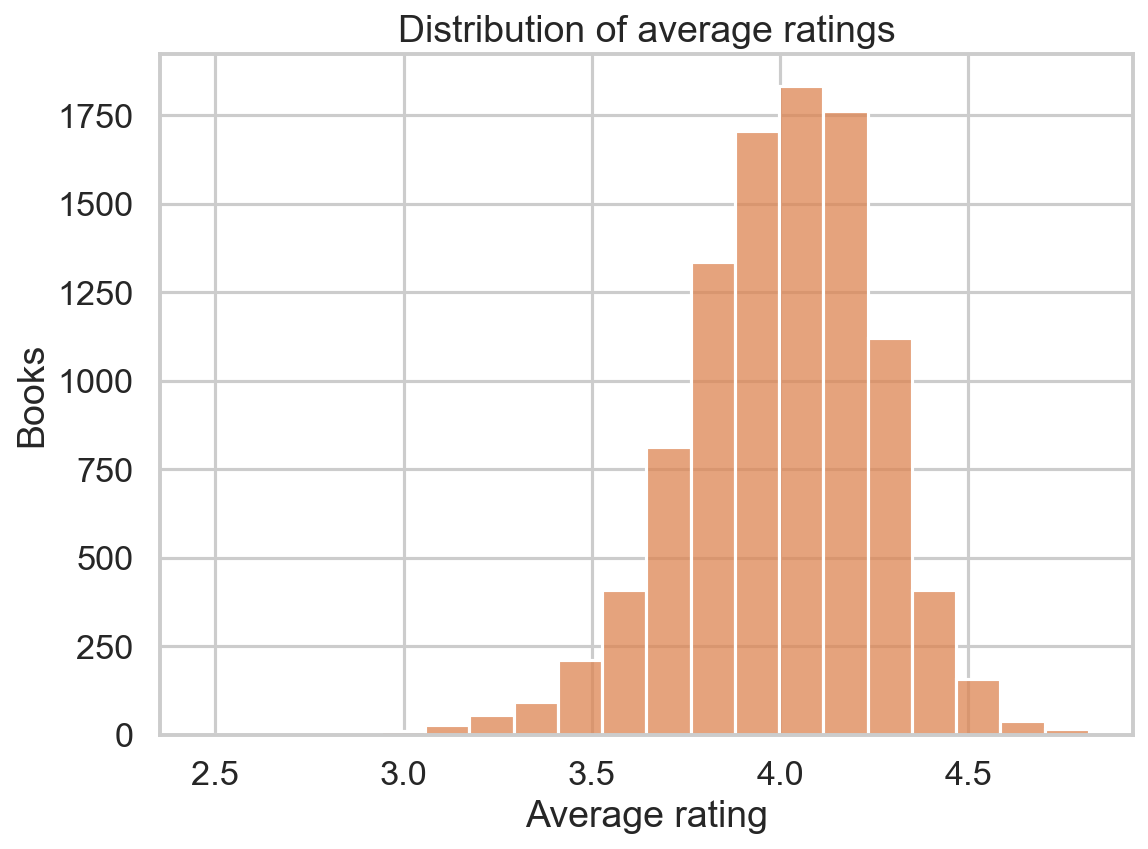
\includegraphics[width=.8\linewidth]{average_rating_hist.png}}{\begin{center}\textit{average\_rating\_hist.png was unavailable at build time.}\end{center}}
    \caption{Distribution of average item ratings informs implicit confidence scaling.}
    \label{fig:avg-rating-hist}
\end{figure}

\dataStatusNote
